\documentclass[11pt]{article}\usepackage[]{graphicx}\usepackage[]{color}
%% maxwidth is the original width if it is less than linewidth
%% otherwise use linewidth (to make sure the graphics do not exceed the margin)
\makeatletter
\def\maxwidth{ %
  \ifdim\Gin@nat@width>\linewidth
    \linewidth
  \else
    \Gin@nat@width
  \fi
}
\makeatother

\definecolor{fgcolor}{rgb}{0.345, 0.345, 0.345}
\newcommand{\hlnum}[1]{\textcolor[rgb]{0.686,0.059,0.569}{#1}}%
\newcommand{\hlstr}[1]{\textcolor[rgb]{0.192,0.494,0.8}{#1}}%
\newcommand{\hlcom}[1]{\textcolor[rgb]{0.678,0.584,0.686}{\textit{#1}}}%
\newcommand{\hlopt}[1]{\textcolor[rgb]{0,0,0}{#1}}%
\newcommand{\hlstd}[1]{\textcolor[rgb]{0.345,0.345,0.345}{#1}}%
\newcommand{\hlkwa}[1]{\textcolor[rgb]{0.161,0.373,0.58}{\textbf{#1}}}%
\newcommand{\hlkwb}[1]{\textcolor[rgb]{0.69,0.353,0.396}{#1}}%
\newcommand{\hlkwc}[1]{\textcolor[rgb]{0.333,0.667,0.333}{#1}}%
\newcommand{\hlkwd}[1]{\textcolor[rgb]{0.737,0.353,0.396}{\textbf{#1}}}%

\usepackage{framed}
\makeatletter
\newenvironment{kframe}{%
 \def\at@end@of@kframe{}%
 \ifinner\ifhmode%
  \def\at@end@of@kframe{\end{minipage}}%
  \begin{minipage}{\columnwidth}%
 \fi\fi%
 \def\FrameCommand##1{\hskip\@totalleftmargin \hskip-\fboxsep
 \colorbox{shadecolor}{##1}\hskip-\fboxsep
     % There is no \\@totalrightmargin, so:
     \hskip-\linewidth \hskip-\@totalleftmargin \hskip\columnwidth}%
 \MakeFramed {\advance\hsize-\width
   \@totalleftmargin\z@ \linewidth\hsize
   \@setminipage}}%
 {\par\unskip\endMakeFramed%
 \at@end@of@kframe}
\makeatother

\definecolor{shadecolor}{rgb}{.97, .97, .97}
\definecolor{messagecolor}{rgb}{0, 0, 0}
\definecolor{warningcolor}{rgb}{1, 0, 1}
\definecolor{errorcolor}{rgb}{1, 0, 0}
\newenvironment{knitrout}{}{} % an empty environment to be redefined in TeX

\usepackage{alltt}
\usepackage[T1]{fontenc}

\usepackage{fullpage}
\usepackage{url}
\usepackage{hyperref}
\usepackage{graphicx}
%\usepackage{underscore}


%
% Obtaining data (8 points total): 
% 2 pts: documentation of how data was obtained (newly assembled or existing
% data) + source code if applicable
% 2 pts: explanation of criteria for inclusion of nodes and edges
% 4 pts: subjective interestingness/originality of the subject of data collection
%
% Data analysis (17 points total):
% 3 pts: were at least 3 metrics/methods from the course applied to the data?
% 4 pts: were they applied/interpreted appropriately?
% 2 pts: was at least one additional technique, not covered in the course
% materials, applied to the data?
% 5pts Visualization: Did the visualization add to your comprehension of the data?
% 3 pts: was code/step by step instructions provided such that one could
% replicate the methods?
%
% Interpretation (5 points): 
% 2pts: were limitations of the data correctly addressed?
% 3pts: did the analysis yield new insights (subjective)
%
\IfFileExists{upquote.sty}{\usepackage{upquote}}{}
\begin{document}

\title{Social Network Analysis of NFL Coaches, 1980-2013}
\author{Nathan E Dire}
\date{November 2014}
\maketitle

\section{Introduction}

Coaching in the United States' National Football League is a high stakes
business.  NFL coaches domainate the top paid coaches in U.S. sports
\cite{forbes-pay}.  The best coaches are paid in excess of \$7 million per year.

The group of NFL coaches is a relatively tight circle.  Head coaches are often
hired from the pool of offensive and defensive coordinators.  

The There is general perception that influential coaches pass on their knowledge to
assistants, who then become successful head coaches themselves.
\begin{figure}
\begin{center}
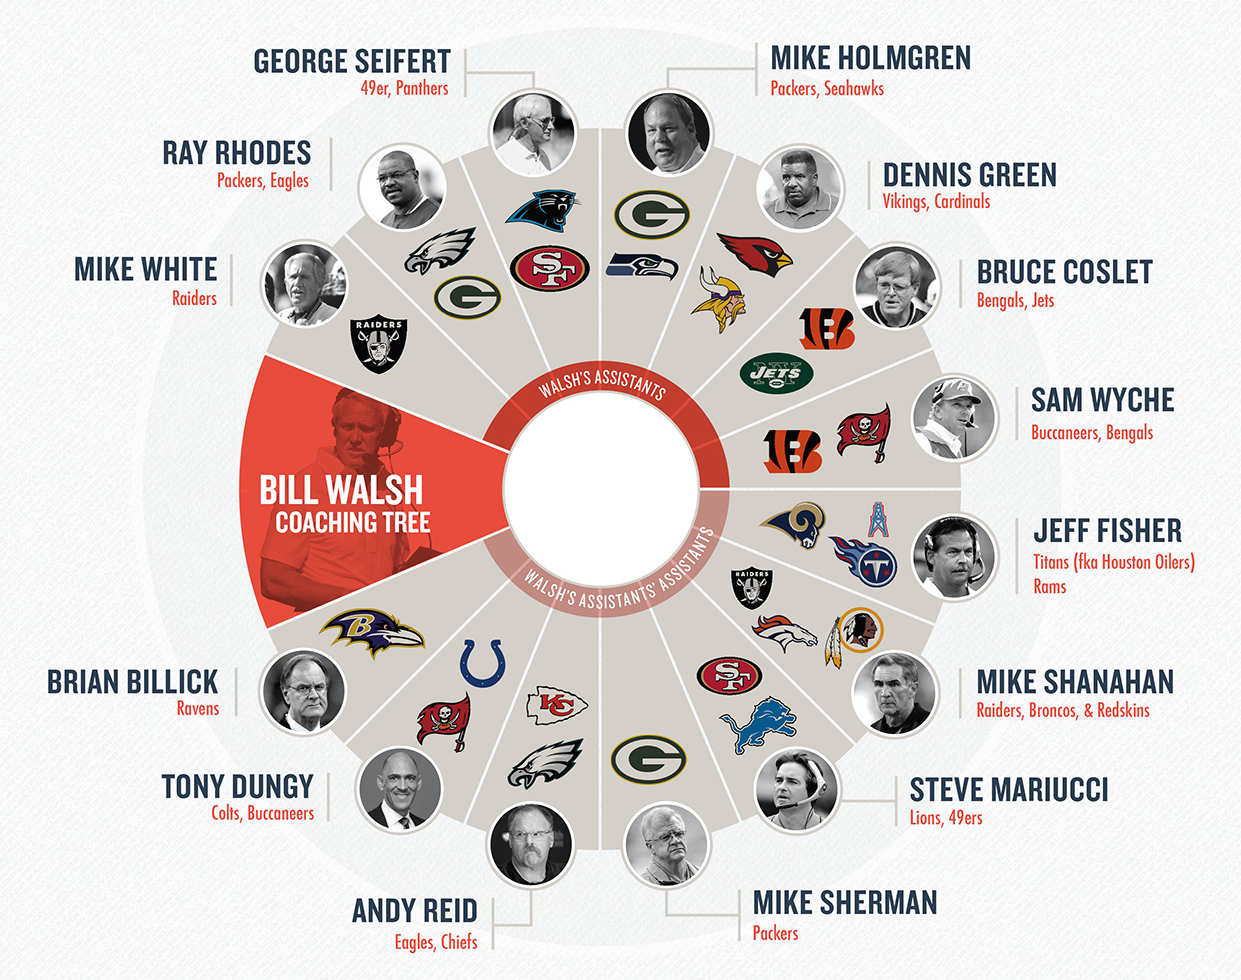
\includegraphics[width=\textwidth]{walsh_network.png}
\end{center}
\caption{Image: The Bill Walsh Coaching Tree. Source:
\url{http://blog.hubspot.com/marketing/paypal-mafia-bill-walsh-nfl-infographic}}
\label{fig-bill-walsh}
\end{figure}

This report considers a few main questions about NFL coaches who have worked
together.  First, does centrality in the social network align with overall
coaching success?  Are there communities in the network?  Small world
characteristics?

\section{Methodology}

\subsection{Data Acquisition}

Data on NFL coaching staffs was gathered from the site
\url{http://www.pro-football-reference.org} by reading the pages and parsing
the listed coaching staff.  For example, this page
\url{http://www.pro-football-reference.com/teams/det/2010.htm} lists the
coaches for the 2010 Detroit Lions.  The team page generally lists the head
coach, offensive coordinator, and defensive coordinator.  Only the years
1980-2013 were considered.  The code used to produce this data is available at \cite{scraper}.

\subsection{Network Construction}

The relationship between members of the coaching staff is subject to
interpretation.  Within this data, the coach may be both a coordinator and head
coach.  

For this analysis, I consider two constructions of the social network:
\begin{enumerate}

\item The first model attempts to follow the ``coaching family tree''
perception, and only has directed edges from head coach to coordinator.  This
approach attempts to model the influence of successful coaches through the
success of their assistants.  Edges are between the head coach and the
coordinators; coordinators have no connection to each other.  This model will
be referred to as the \emph{tree} model.  The file is {\tt coaches\_tree.gml}.

\item The second model considers each member of the staff to be connected with
every coach they served with, with increasing weight for each year served.
This approach attempts to identify coaching ``communities'' who may tend serve
together.  This model will be referred to as the \emph{peer} model.  The file
is {\tt coaches\_peer.gml}.

\end{enumerate}

\subsection{Analysis}

Network analysis is done in the R programming language with the {\tt igraph}
package.  The calculations are included in this document using the {\tt knitr}
package.

\subsection{Limitations}

There are several important limitations of this anlaysis:

\begin{itemize}

\item Only the head coach and coordinators are considered.  This represents the
only clean data available from \url{http://pro-football-reference.com}.  It
also avoids the complexities resulting from teams having different names for
the various position coaches.  This has the downside of not recognizing cases
where head coaches and coordinators take jobs as position coaches.

\item Only the years 1980-2013 are considered.  The consistent reporting of
offensive and defensive coordinators appears to start around 1980.  This
results in the network being truncated for coaches employed before and after
1980.

\item Coaches are considered to serve the entire year.  In reality, teams may
occasionally fire coaches mid-year, and coaches may take a leave of absence.

\end{itemize}

\section{Network Properties}



\begin{knitrout}
\definecolor{shadecolor}{rgb}{0.969, 0.969, 0.969}\color{fgcolor}\begin{kframe}
\begin{alltt}
\hlstd{tree_g} \hlkwb{=} \hlkwd{read.graph}\hlstd{(}\hlstr{"coaches_tree.gml"}\hlstd{,}\hlkwc{format}\hlstd{=}\hlstr{"gml"}\hlstd{)}
\hlkwd{summary}\hlstd{(tree_g)}
\end{alltt}
\begin{verbatim}
## IGRAPH U--- 427 777 -- 
## attr: href (v/c), guid (v/c), label (v/c), id (v/n), value (e/n)
\end{verbatim}
\begin{alltt}
\hlstd{tree_deg} \hlkwb{=} \hlkwd{degree.distribution}\hlstd{(tree_g,} \hlkwc{cumulative} \hlstd{=} \hlnum{TRUE}\hlstd{)}
\hlkwd{plot}\hlstd{(tree_deg,}\hlkwc{log}\hlstd{=}\hlstr{"xy"}\hlstd{,}\hlkwc{xlab}\hlstd{=}\hlstr{"degree k"}\hlstd{,}\hlkwc{ylab}\hlstd{=}\hlstr{"P(x) >= k"}\hlstd{,}\hlkwc{cex}\hlstd{=}\hlnum{0.5}\hlstd{)}
\end{alltt}
\end{kframe}

{\centering \includegraphics[width=\maxwidth]{figure/tree_prop-1} 

}



\end{knitrout}

\begin{knitrout}
\definecolor{shadecolor}{rgb}{0.969, 0.969, 0.969}\color{fgcolor}\begin{kframe}
\begin{alltt}
\hlstd{peer_g} \hlkwb{=} \hlkwd{read.graph}\hlstd{(}\hlstr{"coaches_peer.gml"}\hlstd{,}\hlkwc{format}\hlstd{=}\hlstr{"gml"}\hlstd{)}
\hlkwd{summary}\hlstd{(peer_g)}
\end{alltt}
\begin{verbatim}
## IGRAPH U--- 427 1244 -- 
## attr: href (v/c), guid (v/c), label (v/c), id (v/n), value (e/n)
\end{verbatim}
\begin{alltt}
\hlstd{peer_deg} \hlkwb{=} \hlkwd{degree.distribution}\hlstd{(tree_g,} \hlkwc{cumulative} \hlstd{=} \hlnum{TRUE}\hlstd{)}
\hlkwd{plot}\hlstd{(peer_deg,}\hlkwc{log}\hlstd{=}\hlstr{"xy"}\hlstd{,}\hlkwc{xlab}\hlstd{=}\hlstr{"degree k"}\hlstd{,}\hlkwc{ylab}\hlstd{=}\hlstr{"P(x) >= k"}\hlstd{,}\hlkwc{cex}\hlstd{=}\hlnum{0.5}\hlstd{)}
\end{alltt}
\end{kframe}

{\centering \includegraphics[width=\maxwidth]{figure/peer_prop__-1} 

}



\end{knitrout}

\section{Centrality}

\subsection{Degree}

\subsection{Betweenness}

\begin{knitrout}
\definecolor{shadecolor}{rgb}{0.969, 0.969, 0.969}\color{fgcolor}\begin{kframe}
\begin{alltt}
\hlstd{bb} \hlkwb{=} \hlkwd{betweenness.estimate}\hlstd{(tree_g,} \hlkwc{v}\hlstd{=}\hlkwd{V}\hlstd{(tree_g),} \hlkwc{directed}\hlstd{=}\hlnum{FALSE}\hlstd{,} \hlkwc{cutoff}\hlstd{=}\hlnum{16}\hlstd{)}
\end{alltt}
\end{kframe}
\end{knitrout}

\begin{knitrout}
\definecolor{shadecolor}{rgb}{0.969, 0.969, 0.969}\color{fgcolor}\begin{kframe}
\begin{alltt}
\hlstd{bb} \hlkwb{=} \hlkwd{betweenness.estimate}\hlstd{(peer_g,} \hlkwc{v}\hlstd{=}\hlkwd{V}\hlstd{(peer_g),} \hlkwc{directed}\hlstd{=}\hlnum{FALSE}\hlstd{,} \hlkwc{cutoff}\hlstd{=}\hlnum{16}\hlstd{)}
\end{alltt}
\end{kframe}
\end{knitrout}

\subsection{Closeness}

\section{Community Structure}

% k-core

% fastgreedy

\section{Small World Network Properties}

% cluster coeffient

% Avg shortest path

\section{Conclusion}

This report analyzed the social network of NFL coaches serving as head coach or
coorindator in the years 1980-2013.

The content used to generate this report can be found at \cite{project}.

\begin{thebibliography}{99}

\bibitem{mobility1} Harrison, C.K. \& Associates (2013). Coaching Mobility (Volume I in the Good Business Series). A Report for the NFL Diversity and Inclusion Series.

\bibitem{mobility3} Harrison, C.K. \& Bukstein, S. (2014). NFL Occupational Mobility Patterns (Volume III). A report for the NFL Diversity and Inclusion “Good Business” Series.

\bibitem{forbes-pay}  \url{http://www.forbes.com/sites/chrissmith/2013/05/22/the-highest-paid-coaches-in-us-sports/}

\bibitem{scraper} \url{https://github.com/ndire/pfr-scraper}

\bibitem{project} \url{https://github.com/ndire/sna-nfl-coaches}

\end{thebibliography}

\end{document}
